% Options for packages loaded elsewhere
\PassOptionsToPackage{unicode}{hyperref}
\PassOptionsToPackage{hyphens}{url}
%
\documentclass[
  12pt,
]{article}
\title{Bike Stations in Boston}
\usepackage{etoolbox}
\makeatletter
\providecommand{\subtitle}[1]{% add subtitle to \maketitle
  \apptocmd{\@title}{\par {\large #1 \par}}{}{}
}
\makeatother
\subtitle{\url{https://github.com/bluedevil28/JohnsonFromuthCohen_ENV872_EDA_FinalProject}}
\author{Laurel Cohen, Jeff Fromuth, Blair Johnson}
\date{}

\usepackage{amsmath,amssymb}
\usepackage{lmodern}
\usepackage{iftex}
\ifPDFTeX
  \usepackage[T1]{fontenc}
  \usepackage[utf8]{inputenc}
  \usepackage{textcomp} % provide euro and other symbols
\else % if luatex or xetex
  \usepackage{unicode-math}
  \defaultfontfeatures{Scale=MatchLowercase}
  \defaultfontfeatures[\rmfamily]{Ligatures=TeX,Scale=1}
  \setmainfont[]{Times New Roman}
\fi
% Use upquote if available, for straight quotes in verbatim environments
\IfFileExists{upquote.sty}{\usepackage{upquote}}{}
\IfFileExists{microtype.sty}{% use microtype if available
  \usepackage[]{microtype}
  \UseMicrotypeSet[protrusion]{basicmath} % disable protrusion for tt fonts
}{}
\makeatletter
\@ifundefined{KOMAClassName}{% if non-KOMA class
  \IfFileExists{parskip.sty}{%
    \usepackage{parskip}
  }{% else
    \setlength{\parindent}{0pt}
    \setlength{\parskip}{6pt plus 2pt minus 1pt}}
}{% if KOMA class
  \KOMAoptions{parskip=half}}
\makeatother
\usepackage{xcolor}
\IfFileExists{xurl.sty}{\usepackage{xurl}}{} % add URL line breaks if available
\IfFileExists{bookmark.sty}{\usepackage{bookmark}}{\usepackage{hyperref}}
\hypersetup{
  pdftitle={Bike Stations in Boston},
  pdfauthor={Laurel Cohen, Jeff Fromuth, Blair Johnson},
  hidelinks,
  pdfcreator={LaTeX via pandoc}}
\urlstyle{same} % disable monospaced font for URLs
\usepackage[margin=2.54cm]{geometry}
\usepackage{longtable,booktabs,array}
\usepackage{calc} % for calculating minipage widths
% Correct order of tables after \paragraph or \subparagraph
\usepackage{etoolbox}
\makeatletter
\patchcmd\longtable{\par}{\if@noskipsec\mbox{}\fi\par}{}{}
\makeatother
% Allow footnotes in longtable head/foot
\IfFileExists{footnotehyper.sty}{\usepackage{footnotehyper}}{\usepackage{footnote}}
\makesavenoteenv{longtable}
\usepackage{graphicx}
\makeatletter
\def\maxwidth{\ifdim\Gin@nat@width>\linewidth\linewidth\else\Gin@nat@width\fi}
\def\maxheight{\ifdim\Gin@nat@height>\textheight\textheight\else\Gin@nat@height\fi}
\makeatother
% Scale images if necessary, so that they will not overflow the page
% margins by default, and it is still possible to overwrite the defaults
% using explicit options in \includegraphics[width, height, ...]{}
\setkeys{Gin}{width=\maxwidth,height=\maxheight,keepaspectratio}
% Set default figure placement to htbp
\makeatletter
\def\fps@figure{htbp}
\makeatother
\setlength{\emergencystretch}{3em} % prevent overfull lines
\providecommand{\tightlist}{%
  \setlength{\itemsep}{0pt}\setlength{\parskip}{0pt}}
\setcounter{secnumdepth}{5}
\ifLuaTeX
  \usepackage{selnolig}  % disable illegal ligatures
\fi

\begin{document}
\maketitle

\newpage

\hypertarget{rationale-and-research-questions}{%
\section{Rationale and Research
Questions}\label{rationale-and-research-questions}}

In the era of the climate crisis, the race is on to find ways to reduce
the greenhouse gas (GHG) emissions connected with every possible modern
activity and sector of the economy. Cities face unique challenges and
opportunities in the realm of sustainability. On a basic level, the
major environmental advantage of a city is in population density: urban
dwellers tend to live in high numbers close together, instead of
enacting the low-density, generally high-carbon-footprint sprawl of the
suburbs. In recent years, many cities of various shapes and sizes---from
New York City to Dallas---have introduced bike-sharing programs, where
users can rent bikes for short periods of time and return them to any
one of assorted docking stations around the city. These programs stand
to offer a wide range of benefits, from better health for users who
increase their exercise to less traffic congestion and air pollution on
the roads from fewer cars driven.

As with any other new amenity, it is worth scrutinizing how and where a
given municipality with bike sharing chooses to make that amenity
available. For our study, we chose to investigate the siting of
bike-sharing stations in Boston. The Census data offered thousands of
variables, of which we selected several: demographic, including family
size and race; financial, including homeownership status and income; and
professional, including employment status and mode of commute to work.
For this analysis, we sought to determine whether the locations of
bike-sharing stations in the city were related to the categories of
people found across census tracts. We chose Boston because its data
availability was robust and all the members of our group have lived in
or near Boston, and we focused on bike sharing programs because several
group members are specifically interested in questions of equity and
access in the world of transportation. Public officials in Boston have
also publicly expressed a desire to make bike sharing available to all,
so our team wondered whether that sentiment was evident in the real
locations of bike stations in the city.

We chose the following question to anchor our inquiry:\\
Are bike sharing stations in Boston equally available across population
groups?

\newpage

\hypertarget{dataset-information}{%
\section{Dataset Information}\label{dataset-information}}

2.1 Data Retrieval

For this analysis, we used data from two different sources. For
population data in Boston, we accessed CSVs from the website of the
United States Census, using the data from the 2016-2020 American
Community Survey (ACS). The ACS is conducted every year and is used to
determine how hundreds of millions of state and federal funds are
distributed annually (Census Bureau 2022). For data on the locations of
bike sharing stations in Boston, we downloaded shape files from the Blue
Bikes Boston website. To pull the Census data into R, we used a package
called tidycensus (Walker 2019, Walker and Herman 2022, Moraga 2022)
that allows for easy manipulation and quick visualizations. The
tidycensus package also allows the user to browse through the tens of
thousands of variables encompassed by the ACS. We added all of the data
files to our project repository. All data and code for this project can
be retrieved from the GitHub repository.

\begin{longtable}[]{@{}
  >{\raggedright\arraybackslash}p{(\columnwidth - 4\tabcolsep) * \real{0.19}}
  >{\raggedright\arraybackslash}p{(\columnwidth - 4\tabcolsep) * \real{0.74}}
  >{\raggedright\arraybackslash}p{(\columnwidth - 4\tabcolsep) * \real{0.07}}@{}}
\caption{Dataset Information}\tabularnewline
\toprule
\begin{minipage}[b]{\linewidth}\raggedright
Data Sources
\end{minipage} & \begin{minipage}[b]{\linewidth}\raggedright
Variables Used
\end{minipage} & \begin{minipage}[b]{\linewidth}\raggedright
Time Period
\end{minipage} \\
\midrule
\endfirsthead
\toprule
\begin{minipage}[b]{\linewidth}\raggedright
Data Sources
\end{minipage} & \begin{minipage}[b]{\linewidth}\raggedright
Variables Used
\end{minipage} & \begin{minipage}[b]{\linewidth}\raggedright
Time Period
\end{minipage} \\
\midrule
\endhead
Analyze Boston-City of Boston & Blue Bike Station Locations & Released
in 2021 \\
American Community Survey-U.S. Census Bureau & Percent of homeowners,
Percent of residents carpooling, Percent of residents driving alone,
Percent of residents using public transporation, Percent White, Percent
Non-White, & 2016-2020 Census \\
\bottomrule
\end{longtable}

2.2 Data Wrangling

We began our analysis by importing data from both of our sources. For
the Census data, we used the tidycensus package to select each of the
variables in question individually. For the bike station data, we
imported the shapefiles we had downloaded from the Blue Bikes Boston
website. Next, we filtered all of the data on the county level from
Suffolk County to the city of Boston. For the bike station data, this
filtering was possible using the city name of Boston. For the
tract-based Census data, this filtering was accomplished by selecting
Boston-specific GEOID numbers. After importing the relevant ACS
variables, we removed the margin of error column from the datasets,
spread the data so the format would be conducive to the combining of
datasets, and converted the raw numbers for several of the values of
interest to percentages. We then converted the Census data to
shapefiles, mapped a few of the Census variables against bike station
locations for an initial look at the data, and combined the datasets
using the ``join'' function to allow for combined regression analysis
later on. The opening visualizations can be found in the ``exploratory
analysis'' section below, along with our first impressions of those
maps.

\newpage

\hypertarget{exploratory-analysis}{%
\section{Exploratory Analysis}\label{exploratory-analysis}}

Following initial wrangling, we produced maps combining the locations of
bike sharing stations and the depictions of certain key variables that
relate to transit equity: income and race. We removed GEOIDs and
neighborhoods that were listed as non-residential zones, as those areas
would confound our analyses relating to homeownership as well as to
commuting patterns. The results of this mapping---which informed our
selection of additional variables that represent parts of the lives of
urban families---can be found in the series of images below.

\hypertarget{figure-1}{%
\subsection{\texorpdfstring{\emph{Figure 1}}{Figure 1}}\label{figure-1}}

\begin{flushleft}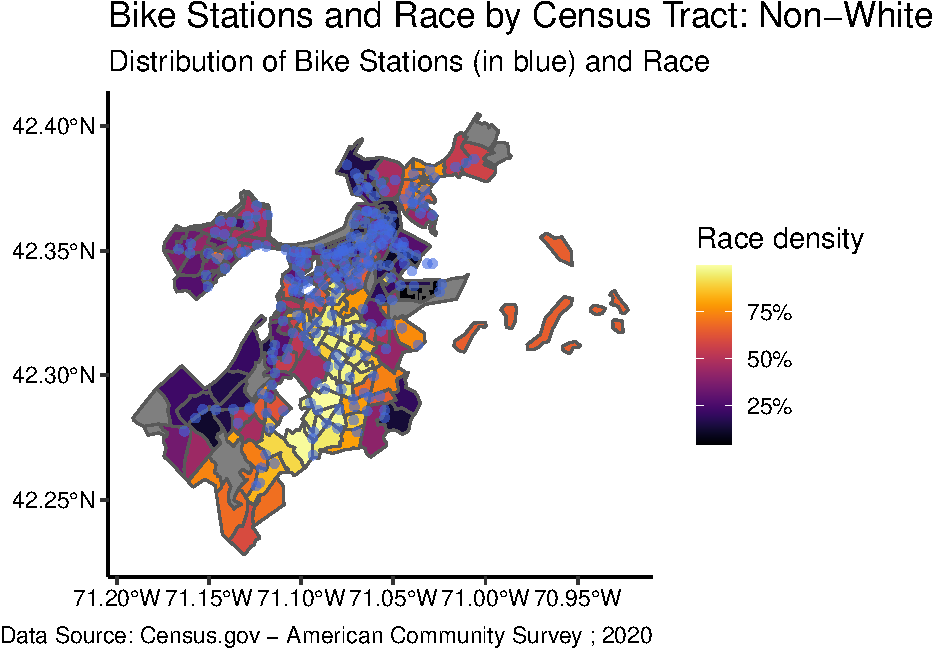
\includegraphics{Project_Template_files/figure-latex/develop plots race non-white-1} \end{flushleft}
\newpage

\hypertarget{figure-2}{%
\subsection{\texorpdfstring{\emph{Figure 2}}{Figure 2}}\label{figure-2}}

\begin{flushleft}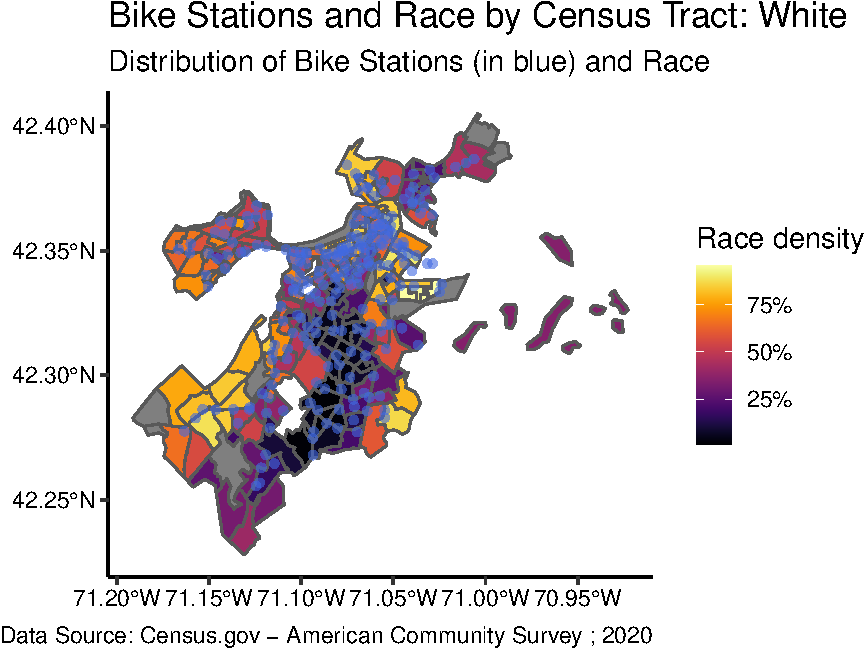
\includegraphics{Project_Template_files/figure-latex/develop plots race white-1} \end{flushleft}

\newpage

\hypertarget{figures-3-and-4}{%
\subsection{\texorpdfstring{\emph{Figures 3 and
4}}{Figures 3 and 4}}\label{figures-3-and-4}}

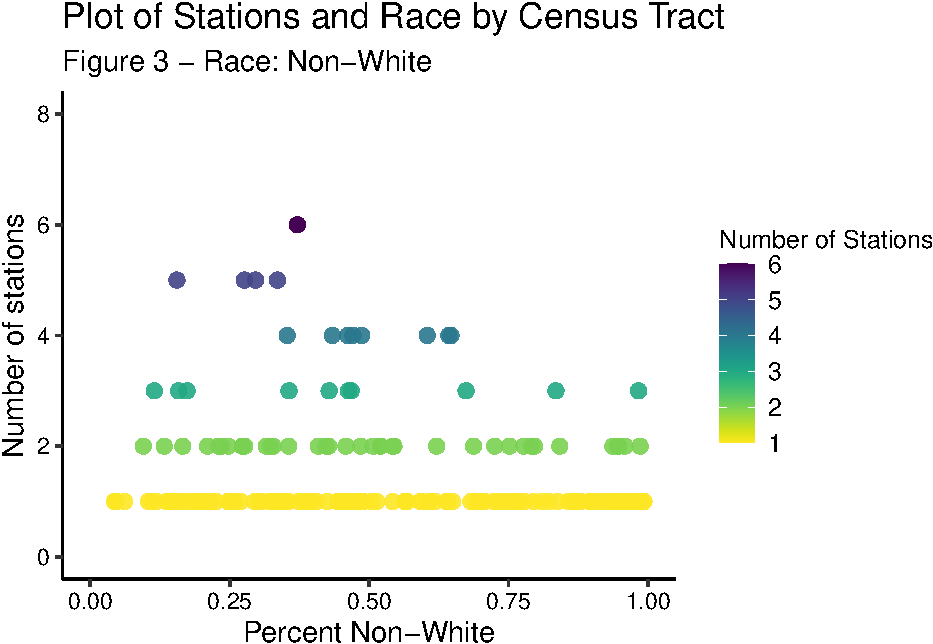
\includegraphics{Project_Template_files/figure-latex/data scatterplots prnnwht-1.pdf}
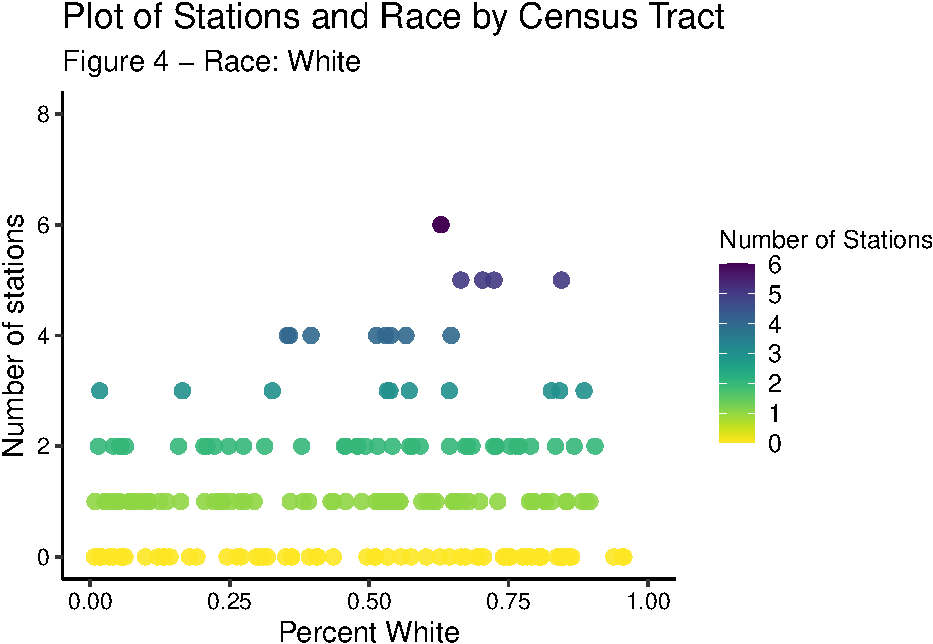
\includegraphics{Project_Template_files/figure-latex/data scatterplots prnnwht-2.pdf}

\hypertarget{figures-5-and-6}{%
\subsection{\texorpdfstring{\emph{Figures 5 and
6}}{Figures 5 and 6}}\label{figures-5-and-6}}

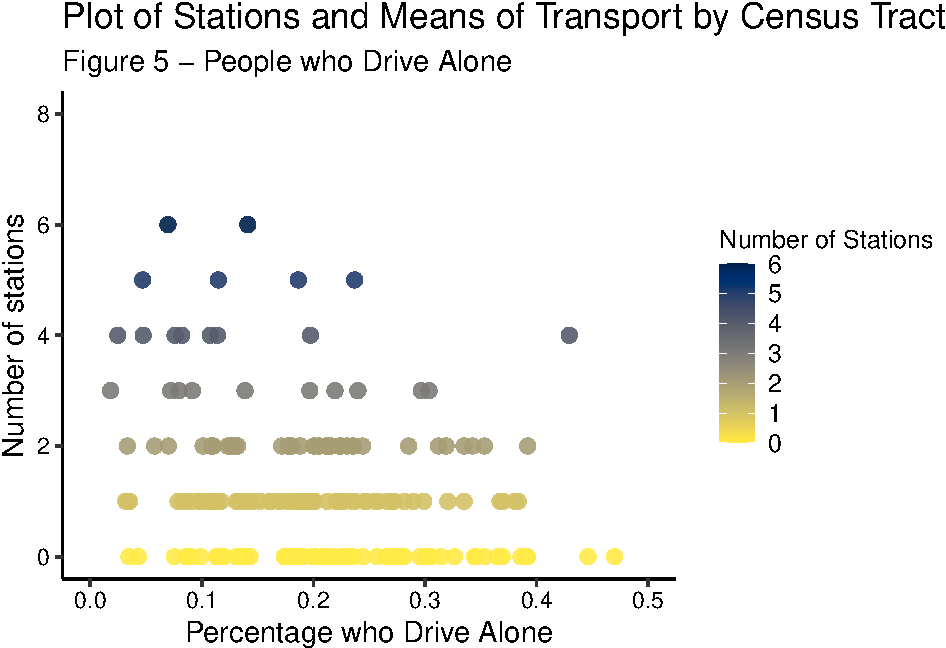
\includegraphics{Project_Template_files/figure-latex/data scatterplots driv_ln-1.pdf}
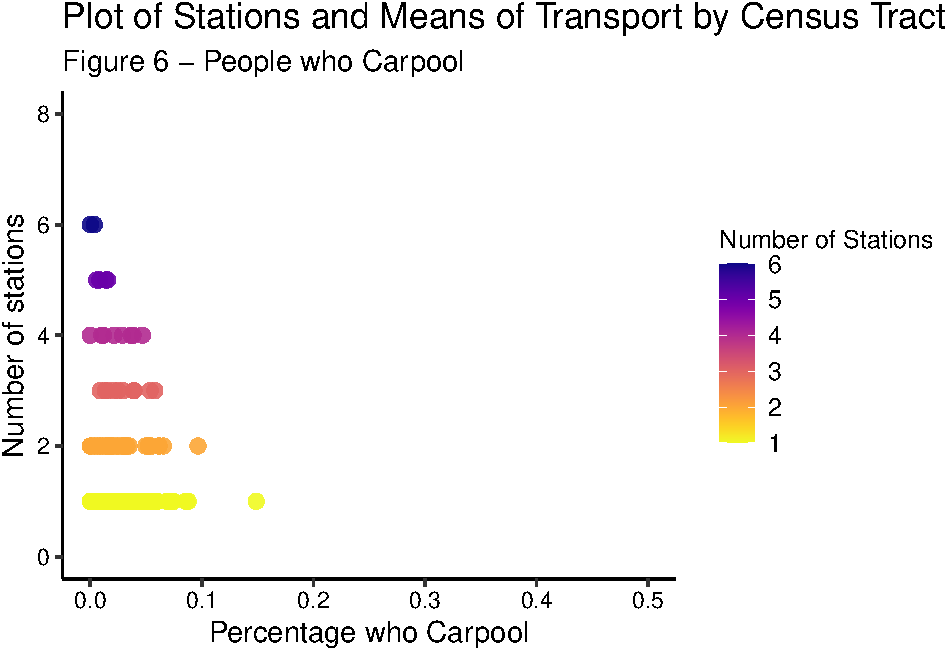
\includegraphics{Project_Template_files/figure-latex/data scatterplots driv_ln-2.pdf}

\hypertarget{figure-7}{%
\subsection{\texorpdfstring{\emph{Figure 7}}{Figure 7}}\label{figure-7}}

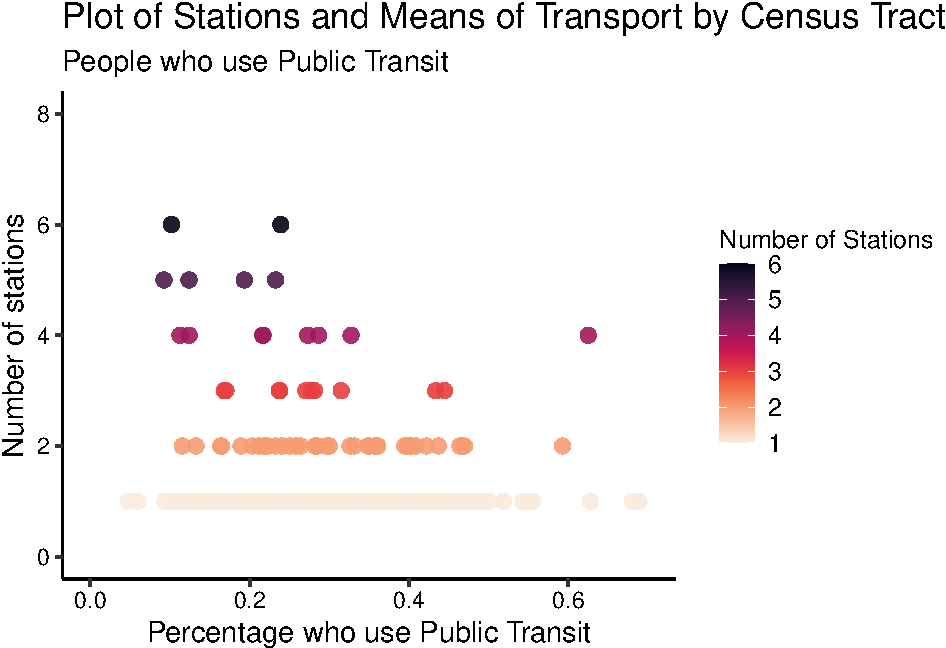
\includegraphics{Project_Template_files/figure-latex/data scatterplots pr_pblc-1.pdf}

\newpage

\hypertarget{analysis}{%
\section{Analysis}\label{analysis}}

\hypertarget{question-are-bike-sharing-stations-in-boston-equally-available-across-population-groups}{%
\subsection{Question: Are bike sharing stations in Boston equally
available across population
groups?}\label{question-are-bike-sharing-stations-in-boston-equally-available-across-population-groups}}

After mapping the most salient equity-related variables against the
locations of bike stations in Boston, we parsed and prepared the other
variables we had selected to be included in a General Linear Model
(GLM). We put all the variables in one dataset and used an Akaike
Information Criterion (AIC) call in R to isolate the variables that
would best contribute to a robust combined regression. Then, we ran a
regression and built a GLM with the strongest variables from the batch
we had chosen. The variables with significance in our final regression
were the percentages of people who use public transit to commute to
work, and who commute to work by driving alone in a personal vehicle. It
is worth noting, though, that the R-Squared values of our regression
were low---0.1293 for the Multiple R-Squared and 0.1055 for the Adjusted
R-Squared---so the proportion of the variation in the locations of bike
stations around Boston that is explained with our selected variables is
low.

\newpage

\hypertarget{summary-and-conclusions}{%
\section{Summary and Conclusions}\label{summary-and-conclusions}}

\hypertarget{expected-distribution-inequity-absent}{%
\subsection{5.1 Expected distribution inequity
absent}\label{expected-distribution-inequity-absent}}

In a typical example of a statistic representing whether bike sharing
programs have been successful in reaching across user groups, one study
found that in New York City, only 16.5\% of people of color have access
to Citi Bike, the city's bike sharing program (Pitt 2019). The
literature also finds that the people who are likeliest to bike to work
are young urban dwellers (US Census Bureau 2019), and ``super-users''
are more likely to be young, have household incomes below \$75,000, and
live and work near bike share stations (Winters et al.~2019). Our team
expected to find similar results in Boston, another city that has
experienced gentrification and the stratification of available amenities
by socio-economic class and race. We did not find such results: both
from the visual and the statistical perspective, demographic variables
like income, race, and age do not have much to do with where bike share
stations are in Boston. These findings could be because the barriers to
participation that we imagined are not the ones that apply. A different
obstacle could be perceptions of cycling safety, although riding a bike
from a bike sharing program can be even safer than riding a personal
bike (Walker 2019). For another idea, one author posits that lack of
information, not access, is what makes bike share programs skew white
and wealthy in many places (Schneider 2017)---in other words, many
people just don't know enough about bike sharing programs to be
comfortable taking advantage of them, despite their ready availability
near where people live.

\hypertarget{alternate-commute-modes-negatively-correlate-with-boston-bike-station-locations}{%
\subsection{5.2 Alternate commute modes negatively correlate with Boston
bike station
locations}\label{alternate-commute-modes-negatively-correlate-with-boston-bike-station-locations}}

The variables that were significant in our regression of Boston bike
station locations were the proportion of people who commute to work via
public transit, and the portion who drive to work alone in a private
car. For both variables, the coefficient in the regression was negative:
-2.3843 at p = 0.000332 for public transit commuters, and -2.1573 at p =
0.027758 for those who drive to work in cars by themselves. Our model
shows that the more people there are in a given census tract who commute
to work either alone in personal vehicles or by public transit, the
lower number of bike stations found in that census tract. This finding
is not what we ancticipated: we posited that there would be a bundling
of pro-environment indicators--more people using environmentally
friendly commuting methods like public transit correlating with more
bike stations available for people to use for errands, recreation, or
commuting. Instead, the two significant variables in the regression
point in opposite directions: fewer bike stations as more people commute
to work alone in private cars (the bundling we expected), but also fewer
bike stations as more people commute to work using public transit (not
the bundling we expected). Perhaps the locations of Boston bike stations
are irrespective of population characteristics altogether, and instead
track other elements of the city, such as areas that are most popular
with tourists. Also, the dataset we used for carpooling behavior was
much smaller than we had hoped, raising the question of whether its
sample size is sufficiently large to merit statistical confidence in the
associated findings.

The larger environmental context around bike sharing programs asks
whether these programs reduce the number of miles that urban residents
drive, as people switch between driving and other modes of transport for
their daily activities. Considering transportation is responsible for
27\% of 2020 GHG emissions in US (EPA 2022), this question is an urgent
one. Bike share programs have been found to reduce car use in some
cities, but not all---and the effectiveness of bike share programs in
protecting the environment is ``dependent on whether {[}these programs
replace{]} car use'' (Fishman et al.~2014). With that said, bike share
programs are most effective at curbing GHGs when they catalyze other
changes, like increases in private bike use, improvements to bicycle
infrastructure, and support of other policies that facilitate cycling
(Schmidt 2018).

\hypertarget{limitations}{%
\subsection{5.3 Limitations}\label{limitations}}

The data we used is from the 5-year estimate from 2016-2019; therefore,
this estimate primarily includes data from before the COVID-19 pandemic
struck. Usage patterns have certainly changed since the pandemic---in
some temporary, and some likely permanent, ways---and in fact there have
been analyses performed on these changes. Because our analysis sought to
investigate the baseline structure of the system, we worked with data
from before the pandemic, but COVID-19 has transformed our society
forever, so those changes are important to consider in future planning
efforts.

Over the course our project, we encountered two primary analytical
difficulties. The first was comparing results across regressions. A
given independent variable might be significant in one regression and
not significant in the other, even though the dependent variable of bike
station locations was the same between both models. We could understand
how the coefficient and significance might vary based on the other
variables in the model, but it did not make sense to us that a variable
that was statistically significant in one analysis could wholly drop
from the statistically significant view in another model with the same
outcome variable. The other analytical issue we faced was the types of
variables available to us. The tidycensus package allows users to access
and analyze the Census data quickly and easily, but it doesn't, of
course, change what kinds of variables the Census includes. Even with
our fairly wide distribution of variables, we still only explained about
10\% of the variation in bike station locations in Boston. With more
kinds of variables---say about land use types, business openings and
closures, or consumer expenditures---we might capture more of the
dynamics that help determine where these bike share stations get built.

\hypertarget{future-recommendations}{%
\subsection{5.4 Future Recommendations}\label{future-recommendations}}

As alluded to above, the first area we recommend future research target
is incorporating other Census datasets and variables into this same type
of analysis. Surveys of capital expenditures, retail trade, business
formation and closures, and consumer expenditures could help illuminate
the value flows in Boston that shape policymakers and developers
perceptions and plans.

Secondly, it would be worth looking closely at how bike sharing impacts
the health of user across neighborhoods in Boston. On a simplistic
level, bike share programs improve users' health through more exercise
(Clockston and Rojas-Rueda 2021), but that effect can be tempered by
exposure to air pollution. Measuring the air pollution across different
types of pollutants---especially PM 2.5, the most dangerous
class---would complement the picture of user-level impacts of bike share
programs.

Third and finally, the impact of bike share programs on overall city
congestion would be an interesting direction for future analysis. One
paper describes mixed effects of such programs on congestion in general,
finding that ``larger cities get better off while richer cities get
worse off'' and these programs ``can reduce peak-hour congestion'' (Wang
and Zhou 2017). From both a quality-of-life and a GHG perspective, many
different stakeholders would appreciate insight into the effects of the
Boston Blue Bikes program on the congestion levels in the very packed
city.

\newpage

\hypertarget{references}{%
\section{References}\label{references}}

Bureau, U. C. (2019, May 14). \emph{May 17 is National Bike to Work
Day}. Census.Gov.
\url{https://www.census.gov/library/stories/2019/05/younger-workers-in-cities-more-likely-to-bike-to-work.html}\\
Bureau, U. C. (2022, January 6). \emph{About the American Community
Survey}. Census.Gov.
\url{https://www.census.gov/programs-surveys/acs/about.html}\\
Clockston, R. L. M., \& Rojas-Rueda, D. (2021). Health impacts of
bike-sharing systems in the U.S. \emph{Environmental Research, 202},
111709. \url{https://doi.org/10.1016/j.envres.2021.111709}\\
Fishman, E., Washington, S., \& Narelle, H. (2014). Bike share's impact
on car use: Evidence from the United States, Great Britain, and
Australia. \emph{Transportation Research Part D: Transport and
Environment, 31}, 13--20.
\url{https://doi.org/10.1016/j.trd.2014.05.013}\\
Moraga, P. (2022). \emph{Chapter 2 Spatial data and R packages for
mapping \textbar{} Geospatial Health Data: Modeling and Visualization
with R-INLA and Shiny}. Retrieved April 17, 2022, from
\url{https://www.paulamoraga.com/book-geospatial/sec-spatialdataandCRS.html}\\
Motivate International Inc.~(2022). \emph{Bluebikes System Data}. Blue
Bikes Boston. Retrieved April 17, 2022, from
\url{http://www.bluebikes.com/system-data}\\
Plitt, A. (2019, July 10). Citi Bike fails to serve New Yorkers in
poverty and communities of color: Report. Curbed NY.
\url{https://ny.curbed.com/2019/7/10/20689177/citi-bike-equity-expansion-report}\\
Schmidt, C. (2018). Active Travel for All? The Surge in Public
Bike-Sharing Programs. \emph{Environmental Health Perspectives, 126}(8),
082001. \url{https://doi.org/10.1289/EHP3754}\\
Schneider, B. (2017, July 14). Bike Sharing Still Has a Stubborn
Diversity Gap. \emph{Bloomberg.Com}.
\url{https://www.bloomberg.com/news/articles/2017-07-14/explaining-the-diversity-and-equity-gap-in-bike-sharing}\\
US EPA, O. (2015, December 29). \emph{Sources of Greenhouse Gas
Emissions {[}Overviews and Factsheets{]}}.
\url{https://www.epa.gov/ghgemissions/sources-greenhouse-gas-emissions}\\
Walker, A. (2019, December 16). \emph{How bike share became the decade's
biggest transit success story}. Curbed.
\url{https://archive.curbed.com/2019/12/16/20864145/bike-share-citi-bike-jump-uber}\\
Walker, K. E. (2022). \emph{Chapter 6 Mapping Census data with R
\textbar{} Analyzing US Census Data}. Retrieved April 17, 2022, from
\url{https://walker-data.com/census-r/mapping-census-data-with-r.html}\\
Walker, K., \& Herman, M. (2022). \emph{Basic usage of tidycensus}.
Retrieved April 17, 2022, from
\url{https://walker-data.com/tidycensus/articles/basic-usage.html}\\
Wang, M., \& Zhou, X. (2017). Bike-sharing systems and congestion:
Evidence from US cities. \emph{Journal of Transport Geography, 65},
147--154. \url{https://doi.org/10.1016/j.jtrangeo.2017.10.022}\\
Winters, M., Hosford, K., \& Javaheri, S. (2019). Who are the
`super-users' of public bike share? An analysis of public bike share
members in Vancouver, BC. \emph{Preventive Medicine Reports, 15},
100946. \url{https://doi.org/10.1016/j.pmedr.2019.100946}

\end{document}
